
	\thispagestyle{empty}
	\rule{\linewidth}{1pt}
	
	\vspace{6pt}				%Die Leerzeilen müssen tatsächlich da sein, sonst funktioniert das nicht
	
	\begin{minipage}{0.5\textwidth}
		\begin{flushleft} 
		\Profs
		\end{flushleft}
	\end{minipage}
	\begin{minipage}{0.49\textwidth}
		\begin{flushright}
			Universität Hamburg
		\end{flushright}
	\end{minipage}

	\rule{\linewidth}{1pt}\\
	\begin{center}
		\huge{\textsf{\titel}}\\
\vspace{8pt}
\large{Zusammenfassung}\\
\small{\Autor}\\
\small{(\Version)}
\vspace{8pt}
	\end{center}

\begin{figure}[htbp]
    \centering
    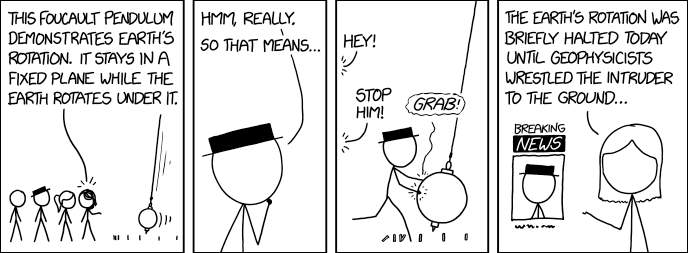
\includegraphics[width=.73\textwidth]{Dateien/Bilder/00xkcd.png}
    \caption*{Bildquelle: \url{https://xkcd.com/2201/}}
\end{figure}
\vfill
\begin{abstract}
\noindent
Moin, dies ist eine informelle Zusammenfassung des Stoffes der Vorlesung \textit{Einführung in die Geophysik}.\\
Die Abbildungen sind der Vorlesung als Screenshots entnommen, ich habe versucht, die wichtigsten Punkte aufzugreifen.\\
Bei Anmerkungen oder Fragen (ich habe bestimmt einige Fehler gemacht) gerne ne Email an fabian.balzer@studium.uni-hamburg.de.\\\\
Viel Erfolg beim Lernen und Üben!\\
:)
\end{abstract}
\cfoot{\pagemark}